\thispagestyle{fancy}
\fancyhead[R]{A.U 2025-2026}
\fancyhead[L]{Chapitre 5 : Sprint 3 -- Conteneurisation et intégration continue}

\chapter{Sprint 3 : Conteneurisation et intégration continue}

% boîte utilisée pour encadrer les extraits de code (verbatim)
\newsavebox{\codebox}

\section*{Introduction}
À l'issue du Sprint 2, la plateforme est fonctionnellement complète mais son déploiement
demeure entièrement manuel : chaque mise à jour impose de se connecter au serveur, de
récupérer le code, d'installer les dépendances et de redémarrer les processus. Cette
procédure est lente, non reproductible et source d'erreurs.

Le \textbf{Sprint 3} répond à cette limite en industrialisant la chaîne de livraison. Il
couvre la conteneurisation de l'ensemble des composants avec Docker, la mise en place
d'un pipeline d'intégration continue sous Jenkins, l'analyse statique de la qualité du
code avec SonarQube et l'analyse des vulnérabilités des images avec Trivy.

L'objectif de ce sprint est qu'un simple \textit{commit} poussé sur le dépôt déclenche
automatiquement la construction, la validation, l'analyse de sécurité et la publication
des images de l'application.

\section{Backlog du Sprint 3}
Les \textit{User Stories} retenues pour ce sprint ont été décomposées en tâches
techniques présentées dans le tableau~\ref{tab:backlog-sprint3}.

\renewcommand{\arraystretch}{1.4}
\begin{longtable}{|>{\raggedright\arraybackslash}p{4.1cm}
                  |>{\raggedright\arraybackslash}p{7.7cm}
                  |>{\centering\arraybackslash}p{2.4cm}|}
\hline
\textbf{User Story} & \textbf{Tâches} & \textbf{Estimation} \\
\hline
\endfirsthead

\hline
\textbf{User Story} & \textbf{Tâches} & \textbf{Estimation} \\
\hline
\endhead

\hline
\multicolumn{3}{r}{\textit{Suite du tableau à la page suivante}} \\
\endfoot

\hline
\caption{Backlog du Sprint 3}
\label{tab:backlog-sprint3}
\endlastfoot

En tant que développeur, je veux conteneuriser le backend.
& Rédiger le \texttt{Dockerfile} du backend (Node.js 20). & 1 \\
& Installer les dépendances en mode production. & 1 \\
& Configurer le gestionnaire de processus PM2 comme point d'entrée. & 1 \\
& Externaliser la configuration par variables d'environnement. & 1 \\
& Tester la construction et l'exécution de l'image. & 1 \\
\hline

En tant que développeur, je veux conteneuriser le frontend.
& Rédiger un \texttt{Dockerfile} multi-étapes (build puis Nginx). & 2 \\
& Configurer Nginx pour le routage côté client. & 1 \\
& Optimiser la taille de l'image finale (base Alpine). & 1 \\
& Tester la construction et l'exécution de l'image. & 1 \\
\hline

En tant que développeur, je veux conteneuriser l'agent de collecte.
& Rédiger le \texttt{Dockerfile} de l'agent (Python 3.11). & 1 \\
& Figer les dépendances dans \texttt{requirements.txt}. & 1 \\
& Tester la collecte depuis le conteneur. & 1 \\
\hline

En tant que développeur, je veux orchestrer les conteneurs en local.
& Rédiger le fichier \texttt{docker-compose.yml}. & 1 \\
& Définir le réseau applicatif et les volumes persistants. & 1 \\
& Configurer les dépendances entre services. & 1 \\
& Tester le démarrage de la pile complète. & 1 \\
\hline

En tant que responsable DevSecOps, je veux automatiser la construction du projet.
& Installer et configurer le serveur Jenkins. & 2 \\
& Créer le \textit{pipeline} déclaratif (\texttt{Jenkinsfile}). & 2 \\
& Configurer le \textit{webhook} GitHub de déclenchement. & 1 \\
& Développer les étapes de récupération et de construction. & 2 \\
& Développer l'étape d'exécution des tests. & 1 \\
& Tester le déclenchement automatique. & 1 \\
\hline

En tant que responsable DevSecOps, je veux mesurer la qualité du code.
& Déployer le serveur SonarQube. & 2 \\
& Rédiger le fichier \texttt{sonar-project.properties}. & 1 \\
& Intégrer l'analyse dans le \textit{pipeline} Jenkins. & 1 \\
& Configurer la \textit{Quality Gate} bloquante. & 2 \\
& Corriger les anomalies remontées par l'analyse. & 2 \\
& Tester le blocage en cas d'échec. & 1 \\
\hline

En tant que responsable DevSecOps, je veux détecter les vulnérabilités des images.
& Installer l'analyseur Trivy sur l'agent Jenkins. & 1 \\
& Intégrer l'analyse des images dans le \textit{pipeline}. & 1 \\
& Définir les seuils de sévérité bloquants. & 1 \\
& Générer et archiver les rapports d'analyse. & 1 \\
& Corriger les vulnérabilités critiques identifiées. & 2 \\
& Tester l'analyse. & 1 \\
\hline

En tant que responsable DevSecOps, je veux publier les images validées.
& Créer les dépôts d'images sur le registre. & 1 \\
& Stocker les identifiants dans le gestionnaire de secrets Jenkins. & 1 \\
& Développer l'étape de publication avec étiquetage par numéro de build. & 1 \\
& Développer l'étape de nettoyage de l'espace de travail. & 1 \\
& Tester la publication. & 1 \\
\hline

\end{longtable}

\section{Diagramme de cas d'utilisation du Sprint 3}
La figure~\ref{fig:uc-sprint3} présente le diagramme de cas d'utilisation correspondant
aux fonctionnalités développées lors du troisième sprint.

\begin{figure}[H]
\centering
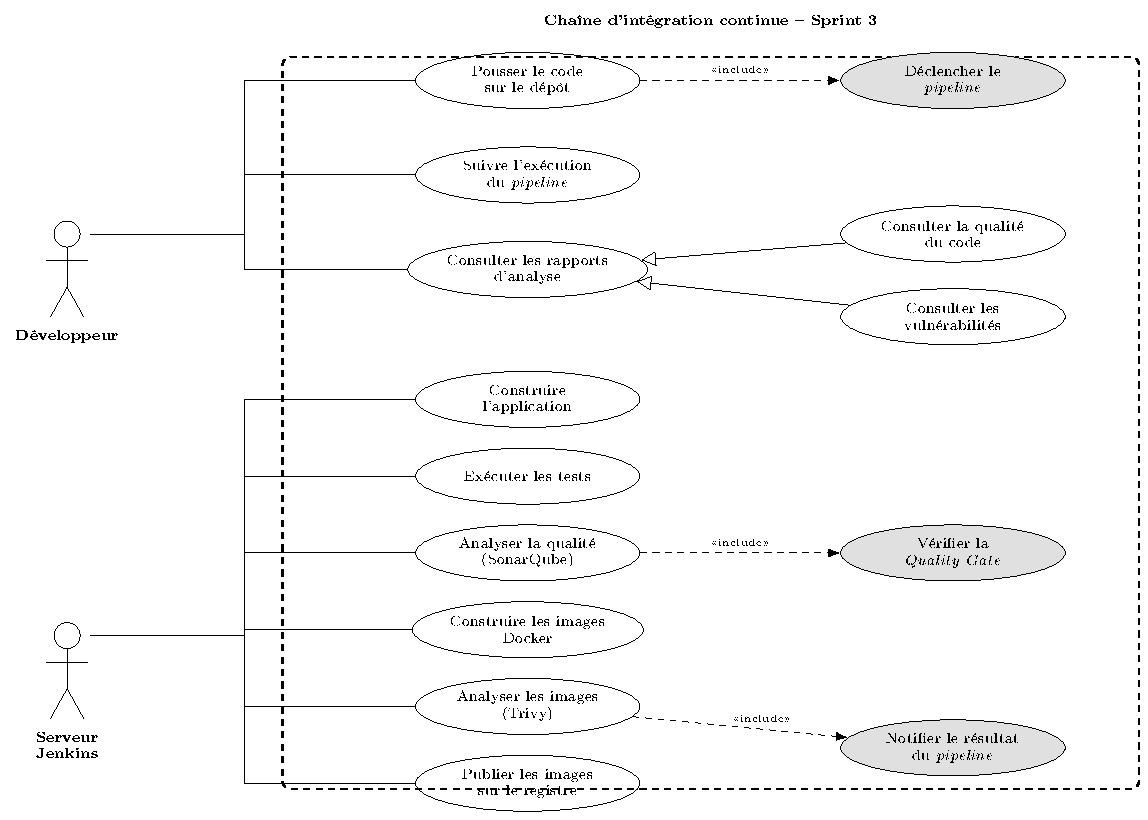
\includegraphics[width=0.96\textwidth]{figures/uc-sprint3.pdf}
\caption{Diagramme de cas d'utilisation du Sprint 3}
\label{fig:uc-sprint3}
\end{figure}

\section{Conteneurisation de l'application}
La conteneurisation consiste à empaqueter une application avec l'intégralité de ses
dépendances dans une unité isolée et portable appelée \textit{image}. Elle garantit que
le comportement observé en développement sera strictement identique en production,
supprimant ainsi la problématique récurrente du « cela fonctionne sur ma machine ».

Trois images distinctes ont été construites, une par composant de la plateforme.

\subsection{Image du backend}
Le backend repose sur l'image officielle \texttt{node:20-slim}. Les dépendances sont
installées en mode production afin d'exclure les outils de développement, et le
gestionnaire de processus PM2 est utilisé comme point d'entrée pour assurer le
redémarrage automatique du service en cas d'incident.

\begin{lrbox}{\codebox}
\begin{minipage}{0.88\textwidth}
\begin{verbatim}
FROM node:20-slim
RUN npm install -g pm2
WORKDIR /app
COPY package*.json ./
RUN npm install --production
COPY . .
EXPOSE 3000
CMD ["pm2-runtime", "server.js"]
\end{verbatim}
\end{minipage}
\end{lrbox}
\begin{figure}[H]
\centering
\fbox{\usebox{\codebox}}
\caption{\texttt{Dockerfile} du backend Node.js}
\label{fig:dockerfile-back}
\end{figure}

\subsection{Image du frontend}
Le frontend fait l'objet d'une construction \textbf{multi-étapes}. La première étape
compile l'application React en fichiers statiques ; la seconde ne conserve que ces
fichiers et les sert par un serveur Nginx léger. Cette approche réduit très
significativement la taille de l'image finale, puisque ni Node.js ni les dépendances de
développement n'y figurent.

\begin{lrbox}{\codebox}
\begin{minipage}{0.88\textwidth}
\begin{verbatim}
FROM node:20-alpine AS build
WORKDIR /app
COPY package*.json ./
RUN npm install
COPY . .
RUN npm run build

FROM nginx:alpine
COPY --from=build /app/build /usr/share/nginx/html
COPY nginx.conf /etc/nginx/nginx.conf
EXPOSE 80
CMD ["nginx", "-g", "daemon off;"]
\end{verbatim}
\end{minipage}
\end{lrbox}
\begin{figure}[H]
\centering
\fbox{\usebox{\codebox}}
\caption{\texttt{Dockerfile} multi-étapes du frontend React}
\label{fig:dockerfile-front}
\end{figure}

\subsection{Image de l'agent}
L'agent de collecte repose sur l'image \texttt{python:3.11-slim}. Les dépendances sont
figées dans le fichier \texttt{requirements.txt} afin de garantir la reproductibilité de
la construction.

\begin{lrbox}{\codebox}
\begin{minipage}{0.88\textwidth}
\begin{verbatim}
FROM python:3.11-slim
WORKDIR /app
COPY requirements.txt ./
RUN pip install -r requirements.txt
COPY . .
CMD ["python3", "main.py"]
\end{verbatim}
\end{minipage}
\end{lrbox}
\begin{figure}[H]
\centering
\fbox{\usebox{\codebox}}
\caption{\texttt{Dockerfile} de l'agent Python}
\label{fig:dockerfile-agent}
\end{figure}

\subsection{Orchestration locale avec Docker Compose}
Afin de reproduire l'environnement complet sur un poste de développement, un fichier
\texttt{docker-compose.yml} décrit l'ensemble des services, le réseau applicatif partagé,
les volumes persistants ainsi que les dépendances de démarrage entre conteneurs. Une
seule commande suffit dès lors à démarrer la totalité de la pile applicative.

\section{Pipeline d'intégration continue}
Le \textit{pipeline} d'intégration continue automatise l'ensemble des opérations
comprises entre la modification du code source et la publication d'une image validée. Il
est décrit de manière déclarative dans un fichier \texttt{Jenkinsfile} versionné avec le
code, ce qui rend la chaîne de livraison elle-même auditable et reproductible.

La figure~\ref{fig:pipeline} illustre l'enchaînement des sept étapes du \textit{pipeline}.

\begin{figure}[H]
\centering
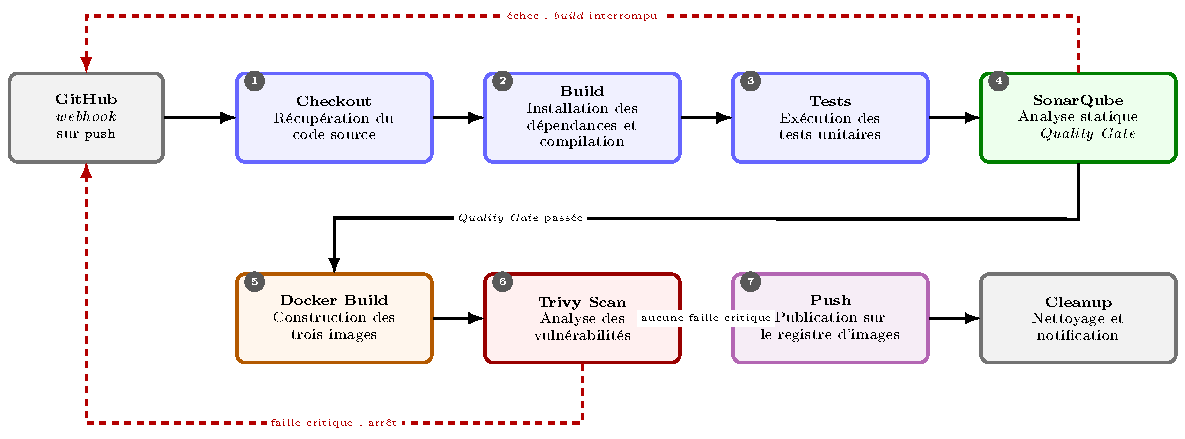
\includegraphics[width=\textwidth]{figures/pipeline.pdf}
\caption{Enchaînement des étapes du \textit{pipeline} Jenkins}
\label{fig:pipeline}
\end{figure}

Le tableau~\ref{tab:stages} détaille le rôle et le critère de succès de chacune de ces
étapes.

\renewcommand{\arraystretch}{1.3}
\small
\begin{longtable}{|>{\centering\arraybackslash}p{1.1cm}
                  |>{\raggedright\arraybackslash}p{2.8cm}
                  |>{\raggedright\arraybackslash}p{5.3cm}
                  |>{\raggedright\arraybackslash}p{4.3cm}|}
\hline
\textbf{N\textsuperscript{o}} & \textbf{Étape} & \textbf{Rôle} & \textbf{Critère de succès} \\
\hline
\endfirsthead

\hline
\textbf{N\textsuperscript{o}} & \textbf{Étape} & \textbf{Rôle} & \textbf{Critère de succès} \\
\hline
\endhead

\hline
\multicolumn{4}{r}{\textit{Suite du tableau à la page suivante}} \\
\endfoot

\hline
\caption{Détail des étapes du \textit{pipeline} d'intégration continue}
\label{tab:stages}
\endlastfoot

1 & \textbf{Checkout} & Récupérer la dernière révision du code source depuis le dépôt GitHub. & Le dépôt est cloné sans erreur. \\
\hline
2 & \textbf{Build} & Installer les dépendances du backend et du frontend, puis compiler l'application React. & La compilation se termine sans erreur. \\
\hline
3 & \textbf{Tests} & Exécuter la suite de tests unitaires du backend. & L'ensemble des tests est en succès. \\
\hline
4 & \textbf{Analyse SonarQube} & Analyser statiquement le code et évaluer la \textit{Quality Gate}. & La \textit{Quality Gate} est franchie. \\
\hline
5 & \textbf{Docker Build} & Construire les images du backend, du frontend et de l'agent, étiquetées par le numéro de build. & Les trois images sont construites. \\
\hline
6 & \textbf{Trivy Scan} & Analyser les images produites à la recherche de vulnérabilités connues. & Aucune vulnérabilité de sévérité critique. \\
\hline
7 & \textbf{Push} & Publier les images validées sur le registre, puis nettoyer l'espace de travail et notifier le résultat. & Les images sont disponibles sur le registre. \\
\hline

\end{longtable}
\normalsize

Le \textit{pipeline} applique le principe du \textbf{\textit{fail fast}} : l'échec d'une
étape interrompt immédiatement l'exécution et notifie l'équipe, évitant qu'un artefact
non conforme ne soit publié. Ce mécanisme constitue le fondement de la démarche
DevSecOps : la sécurité et la qualité ne sont pas contrôlées \emph{après} la livraison,
mais \emph{pendant} la construction.

\section{Analyse de la qualité du code avec SonarQube}
SonarQube réalise une analyse statique du code source, sans l'exécuter, afin d'identifier
quatre familles d'anomalies : les \textit{bugs} potentiels, les vulnérabilités de
sécurité, les \textit{code smells} et la duplication de code. Il mesure également le
taux de couverture par les tests.

La configuration de l'analyse est décrite dans le fichier
\texttt{sonar-project.properties}, présenté dans la figure~\ref{fig:sonar-props}.

\begin{lrbox}{\codebox}
\begin{minipage}{0.88\textwidth}
\begin{verbatim}
sonar.projectKey=monitoring-app
sonar.projectName=DevOps Monitoring App
sonar.sources=.
sonar.exclusions=**/node_modules/**,**/mobile-app/**,**/.git/**
\end{verbatim}
\end{minipage}
\end{lrbox}
\begin{figure}[H]
\centering
\fbox{\usebox{\codebox}}
\caption{Fichier de configuration \texttt{sonar-project.properties}}
\label{fig:sonar-props}
\end{figure}

Une \textbf{\textit{Quality Gate}} bloquante a été configurée : si l'un des indicateurs
franchit le seuil défini, l'étape échoue et le \textit{pipeline} s'interrompt. Les
critères retenus sont présentés dans le tableau~\ref{tab:qualitygate}.

\renewcommand{\arraystretch}{1.3}
\begin{longtable}{|>{\raggedright\arraybackslash}p{6.2cm}
                  |>{\centering\arraybackslash}p{3.4cm}
                  |>{\raggedright\arraybackslash}p{4.5cm}|}
\hline
\textbf{Indicateur} & \textbf{Seuil} & \textbf{Conséquence} \\
\hline
\endfirsthead

\hline
\textbf{Indicateur} & \textbf{Seuil} & \textbf{Conséquence} \\
\hline
\endhead

\hline
\caption{Critères de la \textit{Quality Gate}}
\label{tab:qualitygate}
\endlastfoot

Vulnérabilités de sécurité & 0 & Blocage du \textit{pipeline} \\
\hline
\textit{Bugs} bloquants ou critiques & 0 & Blocage du \textit{pipeline} \\
\hline
Note de maintenabilité & A ou B & Blocage si inférieure \\
\hline
Duplication de code & $<$ 3\,\% & Blocage si dépassée \\
\hline
Points chauds de sécurité revus & 100\,\% & Blocage si incomplet \\
\hline

\end{longtable}

\section{Analyse de sécurité des images avec Trivy}
SonarQube analyse le code écrit par l'équipe, mais une image Docker contient également un
système d'exploitation de base et de nombreuses bibliothèques tierces, qui constituent
une surface d'attaque importante. Trivy comble ce manque en analysant l'image
\emph{construite} : il en inventorie les paquets système et les dépendances applicatives,
puis les confronte aux bases de vulnérabilités publiques.

Deux niveaux de traitement ont été définis :

\begin{itemize}[label=\ding{43}]
  \item les vulnérabilités de sévérité \texttt{CRITICAL} et \texttt{HIGH} interrompent le
        \textit{pipeline} : l'image correspondante n'est jamais publiée ;
  \item les vulnérabilités de sévérité \texttt{MEDIUM} et \texttt{LOW} sont consignées
        dans un rapport archivé par Jenkins et traitées lors des itérations suivantes.
\end{itemize}

Cette analyse a conduit à plusieurs corrections concrètes, notamment le remplacement des
images de base par leurs variantes \texttt{slim} et \texttt{alpine}, nettement plus
légères et donc moins exposées, ainsi que la mise à jour de plusieurs dépendances
transitives présentant des failles connues.

\section{Réalisation du Sprint 3}

\begin{itemize}[label=\ding{220}]
\item \textbf{Images Docker construites :}
\end{itemize}
La figure~\ref{fig:real-images} présente les images produites pour les trois composants
de la plateforme, avec leur taille respective après optimisation.

\begin{figure}[H]
    \centering
    \includegraphics[width=0.9\textwidth]{Image/real-docker-images.png}
    \caption{Images Docker des composants de la plateforme}
    \label{fig:real-images}
\end{figure}

\begin{itemize}[label=\ding{220}]
\item \textbf{Exécution du \textit{pipeline} Jenkins :}
\end{itemize}
La figure~\ref{fig:real-jenkins} illustre la vue d'ensemble du \textit{pipeline} dans
Jenkins. Chaque étape y apparaît avec sa durée d'exécution et son résultat, offrant une
visibilité immédiate sur l'état de la chaîne de livraison.

\begin{figure}[H]
    \centering
    \includegraphics[width=0.95\textwidth]{Image/real-jenkins-pipeline.png}
    \caption{Vue d'ensemble du \textit{pipeline} Jenkins}
    \label{fig:real-jenkins}
\end{figure}

\begin{itemize}[label=\ding{220}]
\item \textbf{Tableau de bord SonarQube :}
\end{itemize}
La figure~\ref{fig:real-sonar} présente le tableau de bord SonarQube du projet. Il
synthétise les indicateurs de qualité, l'état de la \textit{Quality Gate} et le détail
des anomalies détectées.

\begin{figure}[H]
    \centering
    \includegraphics[width=0.95\textwidth]{Image/real-sonarqube.png}
    \caption{Tableau de bord SonarQube du projet}
    \label{fig:real-sonar}
\end{figure}

\begin{itemize}[label=\ding{220}]
\item \textbf{Rapport d'analyse Trivy :}
\end{itemize}
La figure~\ref{fig:real-trivy} illustre le rapport produit par Trivy pour l'image du
backend, détaillant les vulnérabilités identifiées par sévérité ainsi que les versions
correctives disponibles.

\begin{figure}[H]
    \centering
    \includegraphics[width=0.95\textwidth]{Image/real-trivy.png}
    \caption{Rapport d'analyse de vulnérabilités Trivy}
    \label{fig:real-trivy}
\end{figure}

\section*{Conclusion}
Ce chapitre a présenté les travaux réalisés lors du Sprint 3. Celui-ci a permis de
conteneuriser l'intégralité des composants de la plateforme, de mettre en place un
\textit{pipeline} d'intégration continue en sept étapes sous Jenkins, et d'y intégrer
deux barrières de contrôle automatiques : SonarQube pour la qualité du code et Trivy pour
la sécurité des images.

À l'issue de ce sprint, toute modification poussée sur le dépôt est automatiquement
construite, testée, analysée et publiée sans intervention humaine. Le dernier sprint
s'attache désormais au déploiement de ces images sur un cluster Kubernetes selon une
approche GitOps, et à la supervision de l'infrastructure qui les héberge.
